\section{The Design of UPPRESSO}
\label{sec:UPPRESSO}

After we conceptualize the privacy problem into an identifier-transformation problem, the design of UPPRESSO is mainly about designing three identifier-transformation functions to generate pseudo-identifiers for the user and RP as well as linking the user's pseudo-identifier to her account at an RP. In this section, we first present our design of these three functions to support {\em transformed RP designation} and {\em trapdoor user identification} properties, and then describe the details of the UPPRESSO system and its login flow.
%Finally, we discuss the compatibility of UPPRESSO with OIDC.


\subsection{Identifier-transformation Functions in UPPRESSO}
\label{subsec:overview}

%As discussed in Section \ref{sec:challenge}, the identifier-transformation functions are essential for privacy-preserving SSO systems.

We construct three functions, $\mathcal{F}_{ID_{RP} \mapsto PID_{RP}}$, $\mathcal{F}_{ID_{U} \mapsto PID_{U}}$ and $\mathcal{F}_{PID_{U} \mapsto Account}$, based on the NIST elliptic curve $P-256$, 
%the discrete logarithm problem with public parameters $p$, $q$, %and $g$, %% L不作为参数,我们说:e, n是RSA算法参数,不说2048是参数。
where 
%$q$ is a large prime defining the finite field $\mathbb{F}_q$,
$G$ is a point on the curve (known as the base point) 
% $L$ is the length of $q$ in bits,  ($2^{L-1} < q < 2^L$)
and $n$ is the order of the base point $G$. %, and $g$ is a generator of order $q$ in $GF(p)$.
%the prime number $q$  is the order of a multiplicative subgroup of $GF(p)$, which is generated with the generator $g$ by $\{g\ mod\ p, g^2\ mod\ p, ..., g^{q-1}\ mod\ p, 1=g^q\ mod\ p\}$.
The IdP assigns long-term identifiers $ID_U$ and $ID_{RP}$ to a user and an RP respectively, when they first register at the IdP. Without loss of generality, we assume the IdP assigns a unique random number to each user as $ID_U$, where $1<ID_U<n$, and $ID_{RP}$ is a point on the curve generated based on $G$.% For each RP, the IdP selects a random number $r$, where $1 < r < q$, and computes a unique $ID_{RP}$ as:
%\begin{equation}
  %  ID_{RP} = g^{r} \bmod p
   %\label{equ:IDRP}
%\end{equation}
%\noindent where $r$ is kept secret from the RP.

%\vspace{0.5mm}
\noindent {\bf The RP Identifier Transformation Function.} In each login session, the user assists the RP to convert $ID_{RP}$ into a pseudo-identifier $PID_{RP}$. In particular, the user selects a random number $N_{U}$ ($1 < N_{U}<n$) and calculates $PID_{RP}$ as:
%First, the RP chooses a random number $N_{RP}$ ($1 < N_{RP}<q $), and the user chooses another random number $N_{U}$ ($1 < N_{U}<q $).
%Then, they exchange $N_{RP}$ and $N_{U}$ to calculate $PID_{RP}$ following Equation~\ref{equ:PIDRP}.
\begin{equation}
\setlength{\abovedisplayskip}{3pt}
\setlength{\belowdisplayskip}{3pt}
\mathcal{F}_{ID_{RP} \mapsto PID_{RP}}: PID_{RP} = {N_{U}} \cdot {ID_{RP}}
\label{equ:PIDRP}
\end{equation}
With $\mathcal{F}_{ID_{RP} \mapsto PID_{RP}}$,  %satisfies the following requirements.
%is a one-way function so that it 
it is computationally infeasible for the IdP to derive $ID_{RP}$ % from $PID_{RP}$ 
due to the discrete logarithm problem.
Moreover, the nonce $N_{U}$ ensures that: (\emph{a}) $PID_{RP}$ is a one-time pseudo-identifier in each login;  
%that is valid only for the identity proof generated in this login; 
and (\emph{b}) $PID_{RP}$ is dynamically generated in each login. 
When a user visits the same RP multiple times, different $PID_{RP}$s will be generated, which cannot be correlated to the same RP by the curious IdP.


%wo nonces $N_{U}$ and $N_{RP}$ ensure that: (\emph{a}) $PID_{RP}$ is valid only for this login and for the identity proof generated in this login, and (\emph{b}) $PID_{RP}$ is dynamically generated for this login and is different from other $PID_{RP}$s generated in other login session between the same user and RP. Therefore, the IdP cannot associate multiple $PID_{RP}$s of a same RP. Finally, the cooperative generation process between the user and the RP prevents a single malicious entity from manipulating the value of $PID_{RP}$.
%For example, the malicious user fails to make a correct RP accept a $PID_{RP}$ used in another login, while the collusive RPs fail to use a same or correlated $PID_{RP}$s for different logins.


%\vspace{0.5mm}
\noindent {\bf The User Identifier Transformation Function.} 
%Now, the identity proof request to the IdP contains a user identity $ID_U$ and a pseudo-identifier of the RP $PID_{RP}$. Therefore, 
To avoid using the user identity $ID_U$ in identity proofs, the IdP can convert $ID_U$ into a pseudo-identifier for the user as follows:
\begin{equation}
\setlength{\abovedisplayskip}{3pt}
\setlength{\belowdisplayskip}{3pt}
 \mathcal{F}_{ID_{U} \mapsto PID_{U}}: PID_U = {ID_U} \cdot {PID_{RP}}
 \label{equ:PIDU}
\end{equation}
% The function $\mathcal{F}_{ID_{U} \mapsto PID_{U}}$ satisfies the requirements described in Section~\ref{subsec:challenges}.
From Equations%~\ref{equ:IDRP},
~\ref{equ:PIDRP} and~\ref{equ:PIDU}, we see that $PID_U = ({N_UID_U} \bmod n) \cdot {ID_{RP}}$. So, $PID_U$ is a one-time pseudo-identifier. It is only valid in one login session and one identity proof.
As expected, the RP cannot derive $ID_U$ from $PID_U$ due to the discrete logarithm problem, but it can associate a user's one-time pseudo-identifier ($PID_U$) registered at the IdP with her long-term identifier registered at the RP (i.e., $Account$).

%Moreover, although the IdP does not know how the RP identifies the user (i.e. the user's $Account$ at the RP), involving $PID_{RP}$ in the generation of $PID_U$ indirectly links a user's one-time pseudo-identifier at the IdP ($PID_U$) to her long-term identifier at the RP ($Account$) through a trapdoor.

%Moreover, $ID_{RP}$ is generated following Equation~\ref{equ:IDRP} to introduce a random $r$ that is unknown to the RP, so that for a given $ID_U$, $PID_U$ is determined by $r$, $N_{U}$ and $N_{RP}$ together. Otherwise, if two collusive RPs know $r_1$ and $r_2$ respectively, they can check if ${PID_{U_1}}^{r_2N_{U_2}N_{RP_2}} = {PID_{U_2}}^{r_1N_{U_1}N_{RP_1}} \bmod\ p$ holds, which means a same user logs into them in two SSO sessions (i.e., $ID_{U_1}==ID_{U_2}$).

%Moreover, since $r$ is unknown to the RP, collusive RPs cannot link a user's $PID_U$s at different RPs. If $r$ is known to the RP, two collusive RPs might attempt to associate a user's $PID_U$s by checking whether the equality ${PID_{U_1}}^{r_2N_{U_2}N_{RP_2}} = {PID_{U_2}}^{r_1N_{U_1}N_{RP_1}} \bmod\ p$ holds or not, because ${PID_{U_1}} = g^{r_1N_{U_1}N_{RP_1}ID_{U_1}} \bmod p$ and ${PID_{U_2}} = g^{r_2N_{U_2}N_{RP_2}ID_{U_2}} \bmod p$.

%\vspace{0.5mm}
\noindent {\bf The User Account Transformation Function.} We define the trapdoor $T$ in each login session as $T = N_U^{-1} \bmod n$. 
%As $n$ is a prime number and $1< N_U < n$, $n$ is coprime to $N_U$. So, there always exists a $T$ that satisfies $T N_U = 1 \bmod n$. 
With this trapdoor, the RP can easily derive a unique account (denoted as $A$ in the equation) for the user as:%with the function $\mathcal{F}_{PID_{U} \mapsto Account}$
\begin{equation}
\setlength{\abovedisplayskip}{3pt}
\setlength{\belowdisplayskip}{3pt}
   \mathcal{F}_{PID_{U} \mapsto Account}: A = {T} \cdot {PID_U}
   \label{equ:Account}
\end{equation}
From Equations~\ref{equ:PIDRP}, \ref{equ:PIDU} and \ref{equ:Account}, we can further derive:
%\begin{multline}\label{equ:AccountNotChanged}
%   A =  {PID_{U}}^{T}
%   = {({PID_{RP}}^{ID_U})}^{{N_U^{-1} \bmod q}} \\
%   = {ID_{RP}} ^ {ID_U N_U N_U^{-1} \bmod q}
%   = {ID_{RP}}^{ID_U} \bmod p
%\end{multline}
\begin{equation*}
\setlength{\abovedisplayskip}{3pt}
\setlength{\belowdisplayskip}{3pt}
   A =  {T} \cdot {PID_{U}}
%   = {({ID_U})}{{N_U^{-1}){PID_{RP}}}} \\
   = {(ID_U N_U N_U^{-1} \bmod n)} \cdot {ID_{RP}}
   = {ID_U}{ID_{RP}}
   \label{equ:AccountNotChanged}
\end{equation*}
This means when a user logs in to an RP multiple times, the RP can always derive the same $Account$ from different $PID_U$s to uniquely identify the user. However, the RP cannot derive $ID_U$ from $Account$ due to the discrete logarithm problem. 
%Finally, $Account$ provides no clue for different RPs to correlate the users.

With three identifier-transformation functions, UPRESSO supports two desirable properties discussed in Section~\ref{subsec:solutions}
%, namely transformed RP designation and trapdoor user identification,
to satisfy {\em all} the security and privacy requirements of an SSO. %desirable for a secure and privacy-preserving SSO service.
%\vspace{1mm}
%\noindent\textbf{\em Transformed RP designation.}
\begin{comment}
\textbf{\em (i) Transformed RP designation:} using $\mathcal{F}_{ID_{RP} \mapsto PID_{RP}}$, the user and RP cooperatively generate a dynamic $PID_{RP}$ for each login. The identify proof request contains $PID_{RP}$ instead of $ID_{RP}$, so, the RP can verify $PID_{RP}$ is associated with $ID_{RP}$ using the trapdoor but the IdP cannot tell to which RP the user attempts to log in. Also, since $PID_{RP}$s of a same RP are different in different login sessions, the IdP cannot even tell if a same RP is visited.
%Using $PID_{RP}$ and $\mathcal{F}_{ID_{U} \mapsto PID_{U}}$, the IdP generates a corresponding $PID_U$ and encloses it in the identity proof to allow the user to log in to that RP.
%The IdP will bind $PID_{U}$ with $PID_{RP}$ in the identity proof, which designates this identity proof to $PID_{RP}$.
%Therefore, the $PID_{RP}$ is designated to $ID_{RP}$.
%Finally, the transformed RP designation is provided through two phases.
%The function $\mathcal{F}_{ID_{RP} \mapsto PID_{RP}}$ prevents the curious IdP from linking $PID_{RP}$s of different logins at an RP, and
Therefore, it prevents IdP-based login tracing.
%\vspace{1mm}
%\noindent\textbf{Trapdoor User Identification.}
\textbf{\em (ii) Trapdoor user identification:} For each user, different $PID_U$s are generated by the IdP in different login sessions, no matter she requests to log in to a same RP multiple times or to different RPs. However, using $\mathcal{F}_{ID_{U} \mapsto PID_{U}}$ and $\mathcal{F}_{PID_{U} \mapsto Account}$, UPRESSO guarantees that an RP can always derive the unique $Account$ for each user using the dynamically generated $PID_U$ and the corresponding trapdoor in each login session. Meanwhile, collusive RPs cannot link a user's $PID_U$s and $Account$s at different RPs, and therefore prevents RP-based identity linkage.
\end{comment}

\subsection{UPPRESSO Procedures}
\label{implementations}

%\vspace{1mm}
\noindent \textbf{System Initialization.} UPPRESSO consists of four procedures. Firstly, IdP calls system initialization once to establish the system. 
%In particular, the IdP %chooses $L$,
%generates a large prime $p$, and a prime factor $q$ of $p-1$
% and a generator $g$ of order $q$
%as the parameters of the discrete logarithm problem. %~\cite{gallagher2013digital}.
In particular, the IdP generates key pair ($SK$, $PK$) to sign identity proofs and RP certificates.
%The lengths of %$p$, $q$ and 
%($SK$, $PK$) should satisfy the required security strength. 
Then, the IdP keeps $SK$ secret, while announcing %$p$, $q$ and 
$PK$ as public parameters.
%The values of $p$, $q$, $g$ remain the same during the full lifecycle of an SSO system.
%While, the asymmetric key pair ($SK$, $PK$) will be updated when necessary. For example, when $SK$ is leaked, IdP must update ($SK$,$PK$).

%\vspace{1mm}
\noindent\textbf{RP Initial Registration.} Each RP calls an initial registration process once to obtain configurations. In particular, an RP registers itself at the IdP to obtain a unique identifier $ID_{RP}$ and the corresponding RP certificate $Cert_{RP}$ as follows: (i) The RP sends 
a registration request to the IdP, including 
the RP endpoint (e.g., URL) to receive identity proofs; (ii) The IdP generates a unique $ID_{RP}$ and signs $[ID_{RP}, Endpoint_{RP}, *]$ using $SK$, where $*$ denotes supplementary information such as the RP's common name; then, the IdP returns $Cert_{RP} = [ID_{RP}, Endpoint_{RP}, *]_{SK}$ to the RP, where $[\cdot]_{SK}$ means the message is signed using $SK$; (iii) The RP verifies $Cert_{RP}$ using $PK$ and accepts $ID_{RP}$ and $Cert_{RP}$ if they are valid.
%\begin{itemize}
%\item The RP sends a registration request to the IdP, including the RP endpoint (e.g., URL) to receive identity proofs.
%\item The IdP generates the unique generator $ID_{RP}$,
%chooses a unique random number $r$ ($1 < r < q$), calculates $ID_{RP} = g^r \bmod p$,
%signs $[ID_{RP}, Endpoint_{RP}, *]$ using $SK$, where $*$ denotes the supplementary information such as the RP's common name, and returns $Cert_{RP} = [ID_{RP}, Endpoint_{RP}, *]_{SK}$ to the RP, where $[\cdot]_{SK}$ means the message is signed using $SK$.
%\item The RP verifies $Cert_{RP}$ using $PK$ and accepts $ID_{RP}$ and $Cert_{RP}$ if they are valid.
%\end{itemize}
Note that, in UPRESSO, $ID_{RP}$ must be generated by the IdP but cannot be chosen by the RP.% with $r$ unknown to the RP.

%\vspace{1mm}
\noindent\textbf{User registration.} UPPRESSO adopts a similar user registration process as the ones in other SSO systems. Each user registers once at the IdP to set up a unique user identifier $ID_U$ and the corresponding user credential. 
%$ID_U$ can be chosen by the user or the IdP, as long as it is unique for each user.

%\vspace{1mm}
\noindent\textbf{SSO Login.} An SSO login procedure is launched when a user requests to log in to an RP.
%, which calls three identifier-transformation functions following the login flow as shown in Figure~\ref{fig:process}.
%Once a user attempts to log into an RP, the SSO login is initiated.
%We use the OIDC implicit protocol flow as an example, to demonstrate  how to integrate the three functions $\mathcal{F}_{ID_{U} \mapsto PID_{U}}$, $\mathcal{F}_{ID_{RP} \mapsto PID_{RP}}$ and $\mathcal{F}_{PID_{U} \mapsto Account}$ into the typical SSO systems.
It consists of five phases, namely scripts downloading, RP identifier transformation, $PID_{RP}$ registration, identity proof generation, and $Account$ calculation, as shown in Figure~\ref{fig:process}.


\begin{comment}
\begin{figure*}
  \centering
  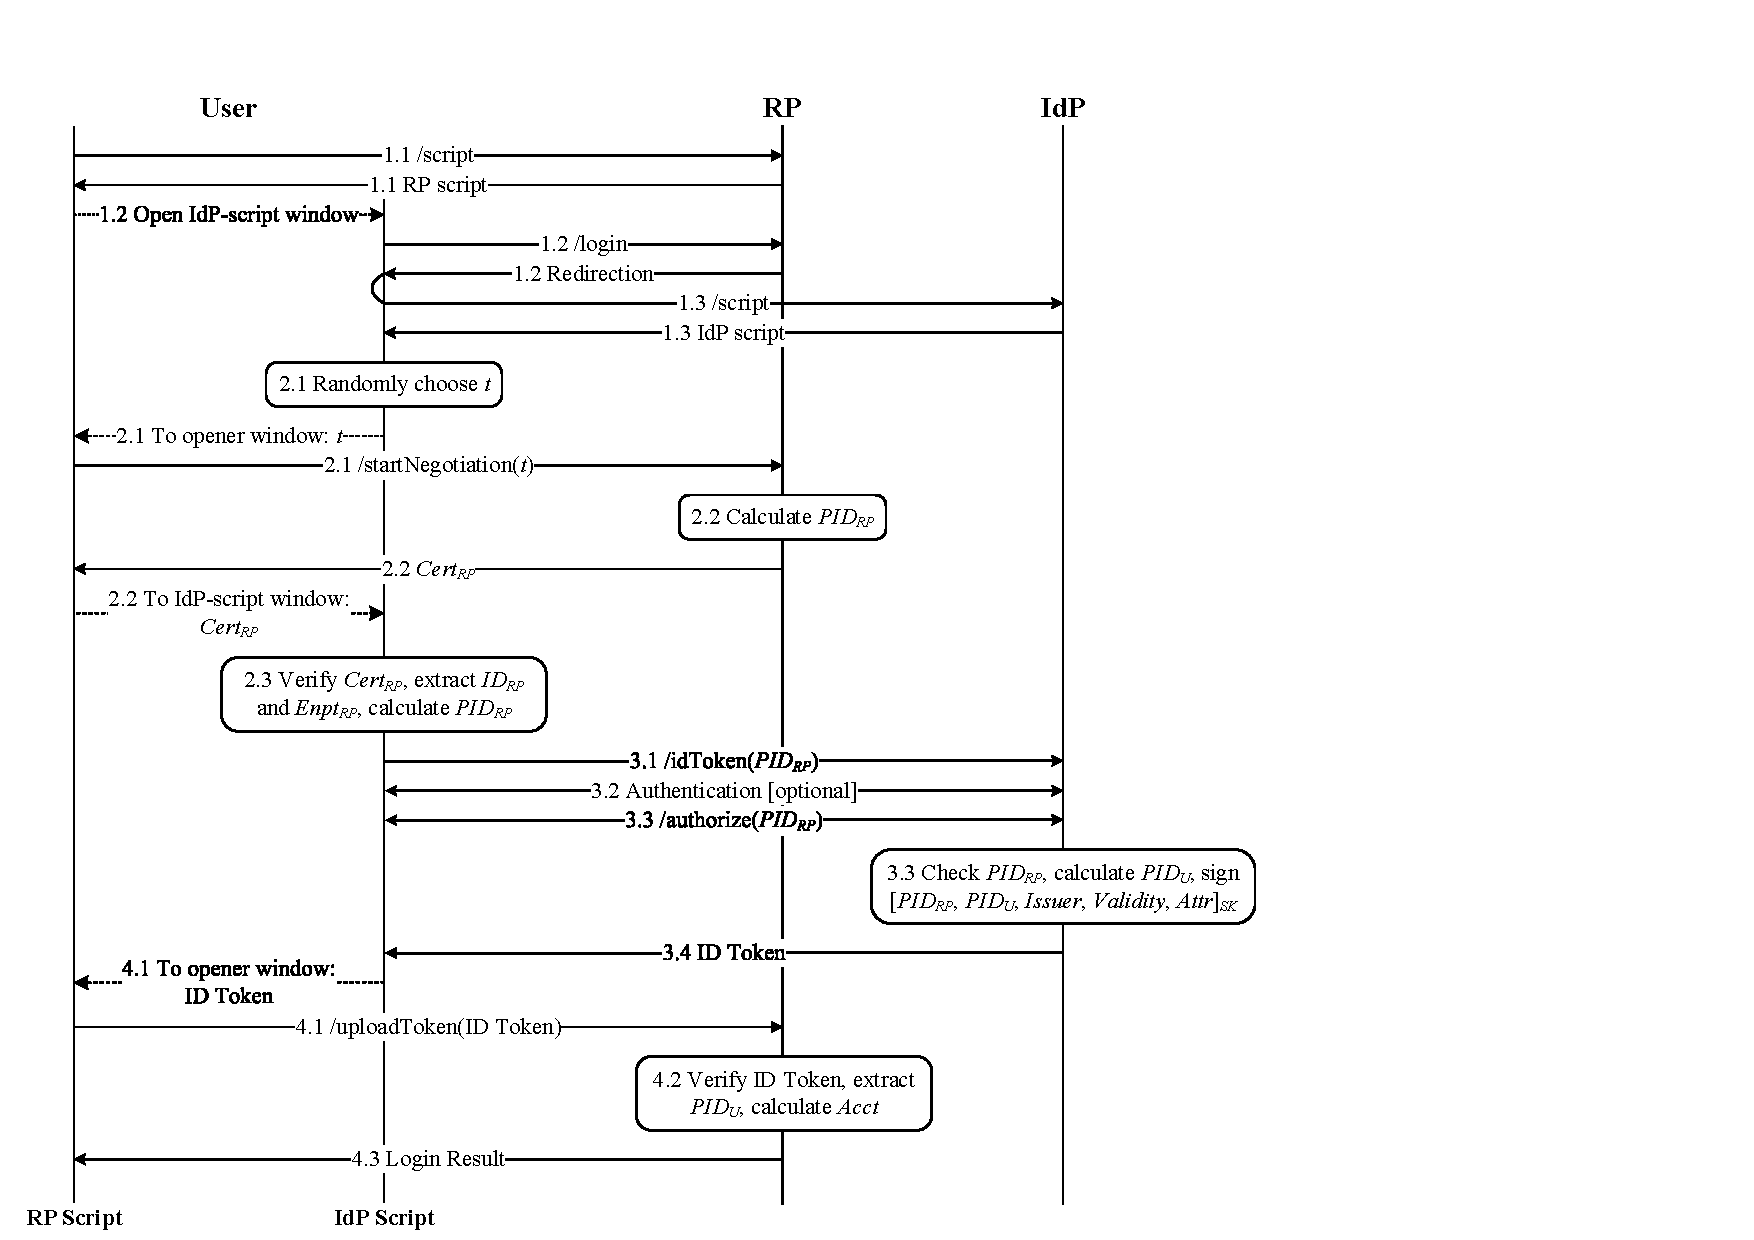
\includegraphics[width=0.9\textwidth]{fig/process-js.pdf}
  \caption{The flow of a user login in UPPRESSO.}
  \label{fig:process}
\end{figure*}
\end{comment}

\vspace{1mm}
\begin{strip}
\centering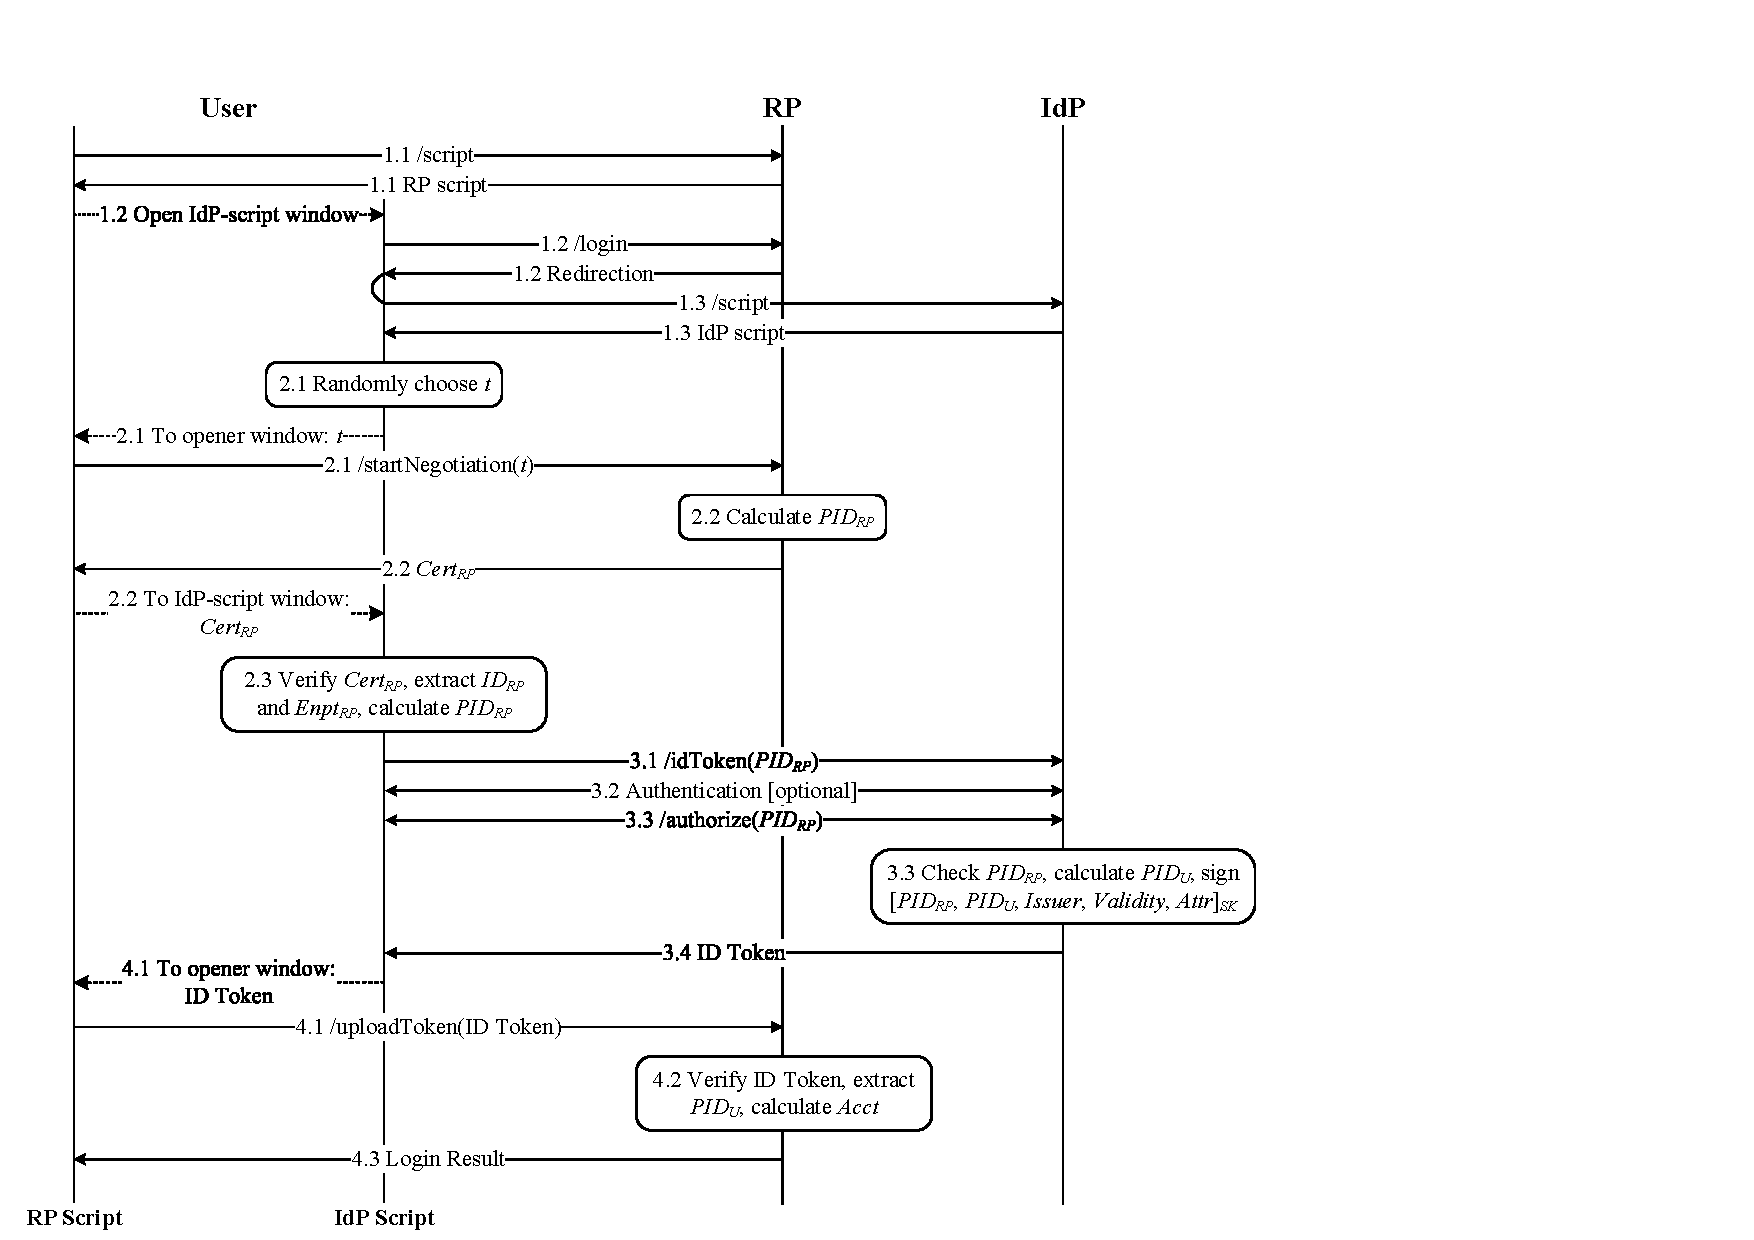
\includegraphics[width=0.9\textwidth]{fig/process-js.pdf}
\captionof{figure}{The flow of a user login in UPPRESSO.}
\label{fig:process}
\vspace{-5mm}
\end{strip}

\noindent{\em 1. Scripts Downloading.}
The scripts downloading phase is for the user's browser to download the scripts from the RP and IdP servers. The browser and two scripts work together to play the user agent role.
\vspace{-\topsep}
\begin{itemize}
%\setlength{\itemsep}{0pt plus 1pt}
\item[1.1] The user visits the RP's site to download the RP script.
\vspace{-\topsep}
\item[1.2] The RP script opens a new window in the browser to visit the login path at the RP server.
\vspace{-\topsep}
\item[1.3] The visit is redirected to the IdP's script site.
\vspace{-\topsep}
\item[1.4] The new window visits the IdP's script site and downloads the IdP script.
\end{itemize}
\vspace{-\topsep}



\noindent{\em 2. RP Identifier Transformation.}
The user and RP cooperate to generate $PID_{RP} = {N_{U}}{ID_{RP}}$. To hide the RP's endpoint from the IdP, the user needs to create a new endpoint to replace the real endpoint of the RP.
\vspace{-\topsep}
\begin{itemize}
%\setlength{\itemsep}{0pt plus 1pt}
\item[2.1] The IdP script chooses a random $N_U$ ($1 < N_U <n$) and sends it to the RP script through postMessage. Then, the RP script sends $N_U$ to the RP server.
\vspace{-\topsep}
\item[2.2] The RP verifies $N_{U} \neq 0 \bmod n$, calculates $PID_{RP}$ and derives the trapdoor $T={N_U}^{-1} \bmod n$. To acknowledge the negotiation of $PID_{RP}$, the RP replies with $Cert_{RP}$, which is transmitted from the RP script to the IdP script through postMessage.
\vspace{-\topsep}
\item[2.3] The IdP script verifies $Cert_{RP}$, extracts $ID_{RP}$ from $Cert_{RP}$ and calculates $PID_{RP}={N_{U}}{ID_{RP}}$ and $nonce=hash(N_U)$. It also creates a one-time endpoint for the RP. If $Cert_{RP}$ is invalid, the user halts the negotiation.
\end{itemize}
\vspace{-\topsep}
It is important to ensure that the RP endpoint is not tampered with by the adversary. In other OIDC systems, the IdP obtains the RP endpoint from RP registration and verifies the endpoint in the identity proof request. However, the IdP in UPPRESSO sees only a one-time endpoint. So, we ask the user to verify the correctness of the RP endpoint using the RP certificate. %which is signed by the IdP.


\noindent{\em 3. $\mathbf{PID_{RP}}$ Registration.}
In this phase, the user registers a new RP with $PID_{RP}$ at the IdP using OIDC's dynamic registration. This step has to be conducted by the user but not the RP. Otherwise, the IdP can associate $PID_{RP}$ and $ID_{RP}$.
\vspace{-\topsep}
\begin{itemize}
%\setlength{\itemsep}{0pt plus 1pt}
\item[3.1] The IdP script sends the $PID_{RP}$ registration request $[PID_{RP}, Hash( N_U), Endpoint_U]$ to the IdP.
\vspace{-\topsep}
\item[3.2] The IdP checks the unexpired $PID_{RP}$s to verify if the received $PID_{RP}$ is unique. Then, it signs the response as $[PID_{RP}, hash( N_U), validity]_{SK}$, where $validity$ denotes when the $PID_{RP}$ will expire.
\vspace{-\topsep}
\item[3.3] The IdP script forwards the registration result to the RP server through the RP script.
\vspace{-\topsep}
\item[3.4] The RP verifies the IdP's signature and accepts the result only if $PID_{RP}$ and $hash(N_U)$ match those in the negotiation and $PID_{RP}$ is not expired.
\end{itemize}
\vspace{-\topsep}
$hash(N_U)$ is a nonce to distinguish different login sessions because there is a very small chance that the same $PID_{RP}$ is generated for two RPs even using two different pairs of $ID_{RP}$s and $N_U$s. This nonce avoids a registration result being acceptable to two RPs.

\noindent{\em 4. ID Proof Generation.}
In this phase, the IdP calculates $PID_U = {ID_U}{PID_{RP}}$ and signs the identity proof. % The processes are as follows.
\vspace{-\topsep}
\begin{itemize}
%\setlength{\itemsep}{0pt plus 1pt}
\item[4.1] The RP constructs an identity proof request containing its $PID_{RP}$ and $Endpoint_{RP}$, which is then forwarded to the IdP script through the RP script.
\vspace{-\topsep}
\item[4.2] The IdP authenticates the user if she has not been authenticated yet.
\vspace{-\topsep}
\item[4.3] First, the user checks the scope of the requested attributes, while the IdP script verifies that $PID_{RP}$ and $Endpoint_{RP}$ in the request are valid. Then, the IdP script replaces the RP's endpoint with the newly registered one-time $Endpoint_U$ and sends the modified identity proof request to the IdP server.
\vspace{-\topsep}
\item [4.4] The IdP verifies if $PID_{RP}$ and $Endpoint_U$ are registered and unexpired, and then calculates $PID_U = {ID_U}{PID_{RP}}$ for the authenticated user.
\vspace{-\topsep}
\item[4.5] The IdP constructs and signs the identity proof $[PID_{RP}, PID_U, Iss, ValTime, Attr]_{SK}$, where $Iss$ is the identifier of the IdP, $ValTime$ is the validity period, and $Attr$ contains the requested attributes.
\vspace{-\topsep}
\item[4.6] The IdP sends the identity proof to the one-time endpoint. The IdP script forwards the identity proof to the RP script that holds the origin $Endpoint_{RP}$. Finally, the RP script sends it to the RP server.
\end{itemize}
\vspace{-\topsep}
In this phase, if any check fails, the process will be halted. For example, the user halts the process if $PID_{RP}$ in the identity proof request is inconsistent with  the negotiated one. The IdP rejects the identity proof request, if the pair of $PID_{RP}$ and $Endpoint_U$ has not been registered.

\noindent{\em 5. $\mathbf{Account}$ calculation.}
The RP verifies the identity proof, derives the user's unique $Account$, and allows her to log in.
\vspace{-\topsep}
\begin{itemize}
%\setlength{\itemsep}{0pt plus 1pt}
\item[5.1] The RP verifies the identity proof, including the signature, validity period, and if $PID_{RP}$ is consistent with the negotiated one. If any fails, the RP rejects this login.
\vspace{-\topsep}
\item [5.2] The RP extracts $PID_U$, calculates $Accout = T \cdot {PID_U}$, and allows the user to log in.
\end{itemize}
\vspace{-\topsep}


\begin{comment}
\subsection{SSO Login Flow of UPPRESSO}
\label{sebsec:loginprocess}

We illustrate the steps of the SSO login protocol of UPPRESSO in Figure~\ref{fig:process}, %the SSO login sub-protocol provides the secure SSO service and prevents both the IdP-based login tracing and RP-based identity linkage.
 % prevents the curious IdP from obtaining the RP's identifying information during the interchanges,
%  and avoids the adversary to break the security and user's privacy.
and describe the detailed processes as follows.

\begin{figure*}
  \centering
  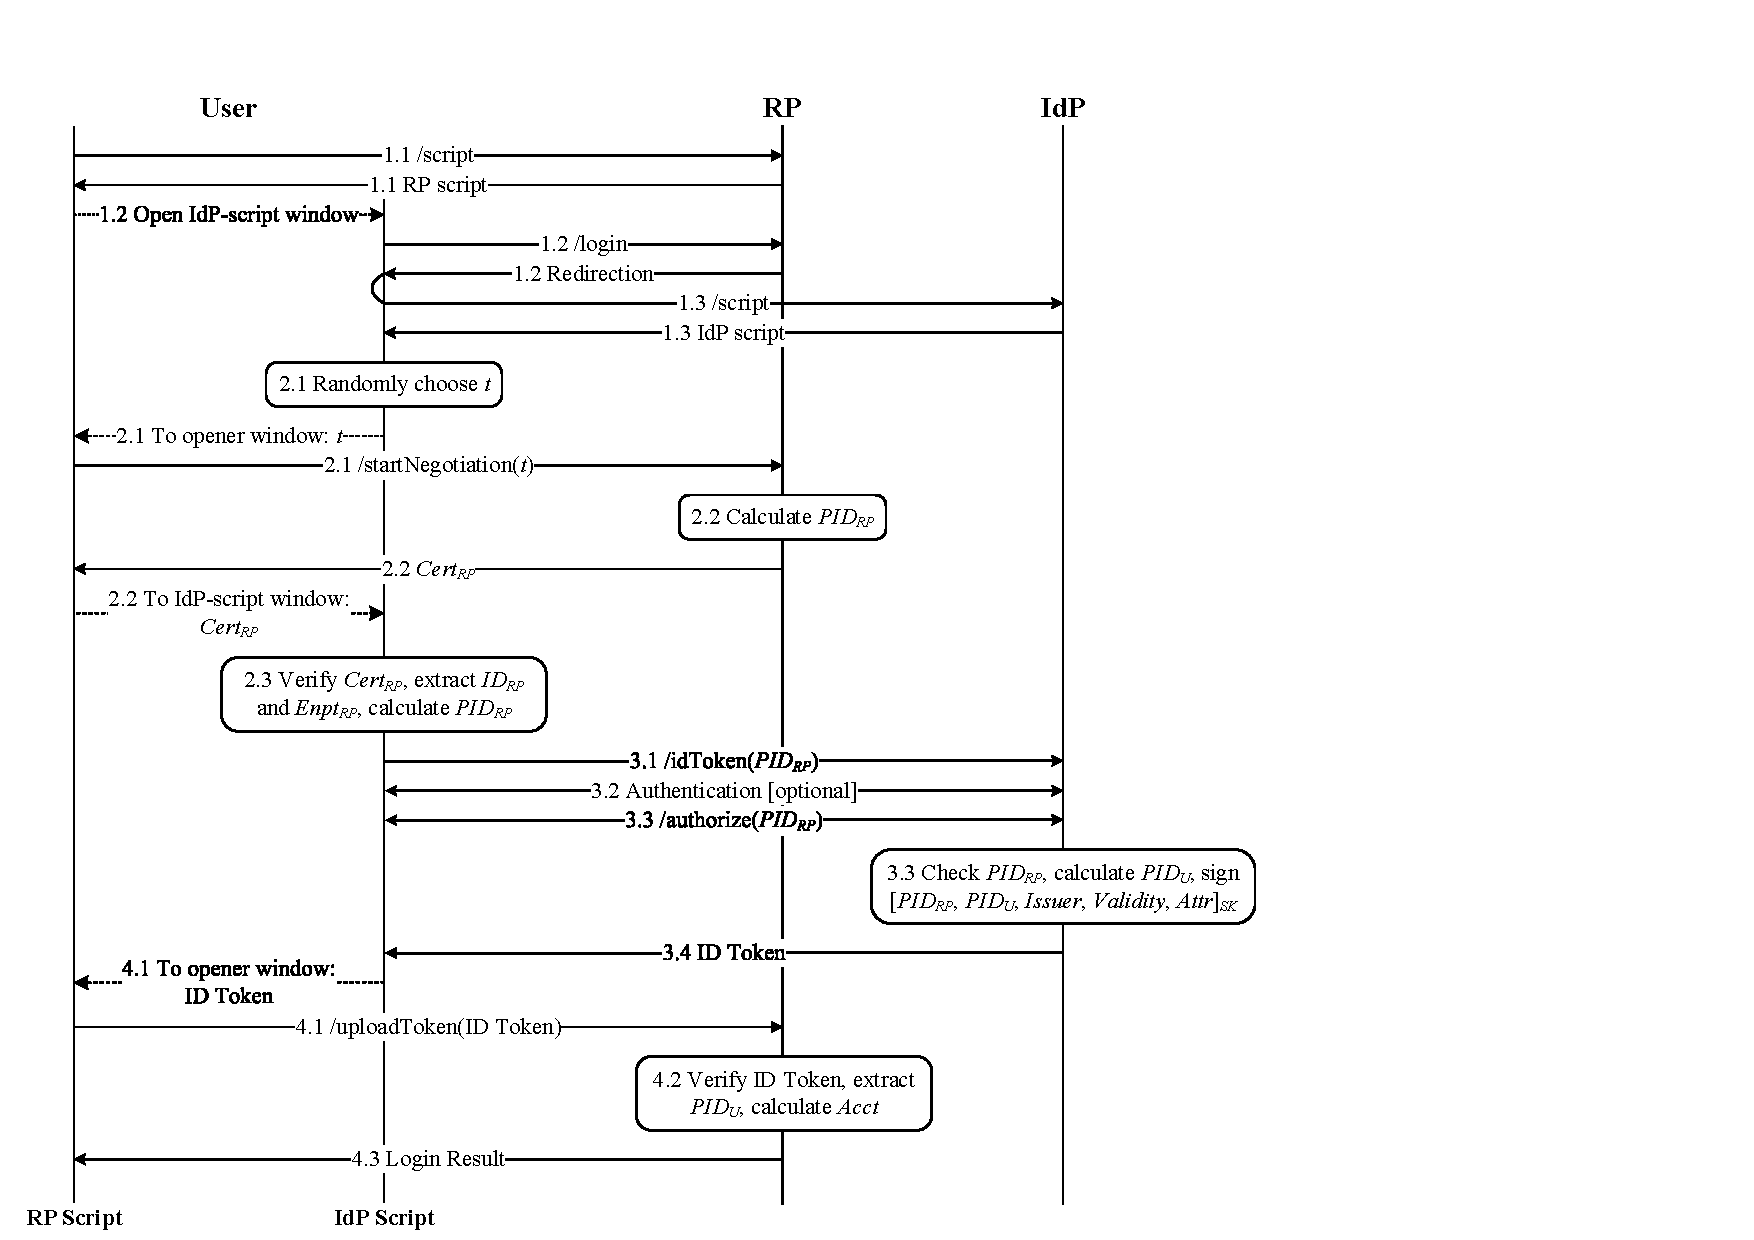
\includegraphics[width=0.68\linewidth]{fig/process-js.pdf}
  \caption{The flow of a user login in UPPRESSO.}
  \label{fig:process}
\end{figure*}

\vspace{1mm}\noindent\textbf{Scripts Downloading.}
At the beginning, the user downloads the scripts from RP server and IdP server as follows:\\

\begin{itemize}
\item[1.1] The user  visits the RP's script site and downloads the script.
\item[1.2] The script opens a new window in the browser visiting the login path at RP server.
\item[1.3] The visit to RP's login path is redirected to IdP's script.
\item[1.4] The new window visits  the IdP's script site and downloads the script.
\end{itemize}

\vspace{1mm}\noindent\textbf{RP Identifier Transformation.}
In this phase, the user and the RP cooperate to generate $PID_{RP}$ as follows:
\begin{itemize}
\item[2.1] The IdP script chooses a random number $N_U$ ($1 < N_U <q$) and sends it to RP script through postMessage, then RP script sends $N_U$ to RP server.
\item[2.2] The RP  verifies $N_{U} \neq 0 \bmod q$, calculates $PID_{RP}$ with $N_U$, derives the trapdoor $T={(N_U N_{RP})}^{-1} \bmod q$; and  acknowledges the negotiation by responding with $Cert_{RP}$. The $Cert_{RP}$ is transmitted from RP script to IdP script through postMessage.
\item[2.3] The IdP script verifies $Cert_{RP}$, extracts $ID_{RP}$ from the valid $Cert_{RP}$,  calculate $PID_{RP}={ID_{RP}}^{N_{U}} \bmod p$, creates a one-time endpoint to hide the RP's endpoint from the IdP and calculates $Nonce=Hash(N_U)$.


 % \item [1.1] The user sends a login request to trigger the negotiation of $PID_{RP}$.
%  \item [1.2] The RP chooses a random number $N_{RP}$ ($1 < N_{RP} <q$), calculates $Y_{RP}={ID_{RP}}^{N_{RP}} \bmod p$, % (Step 2.1.1);
%   and sends $Y_{RP}$ with $Cert_{RP}$  to the user. % (Step 2.1.2).
%  \item [1.3] The user verifies $Cert_{RP}$, extracts $ID_{RP}$ from the valid $Cert_{RP}$, chooses a random number $N_U$ ($1 < N_U <q$) to calculate $PID_{RP}={Y_{RP}}^{N_{U}} \bmod p$, and sends $N_U$ %with $PID_{RP}$
%       to the RP.
%  \item [1.4] The RP verifies $N_{U} \neq 0 \bmod q$, calculates $PID_{RP}$ with $N_U$ and $Y_{RP}$, %checks its consistency with the received one,
 %  derives the trapdoor $T={(N_U N_{RP})}^{-1} \bmod q$; and
%   acknowledges the negotiation by responding with $N_{RP}$.
 % \item [1.5] The user verifies that $N_{RP} \neq 0 \bmod q$ and $Y_{RP} = {ID_{RP}}^{N_{RP}} \bmod p$.
   %sends the calculated $PID_{RP}$ to the user (Step 2.1.6).
%  \item The user checks the consistency of the received $PID_{RP}$ with the stored one.
\end{itemize}

The user halts the negotiation, if  $Cert_{RP}$ is invalid.
%The verification of $Y_{RP}$ and $N_{RP}$ ensures the order of $Y_{RP}$ (and also $PID_{RP}$) is $q$,
  %  and prevents a malicious RP from choosing an arbitrary $Y_{RP}$ (then $PID_{RP}$) of order less than $q$,
    %    which makes it less difficult for the RP to derive $ID_U$ from $PID_U$.
 %or the received $PID_{RP}$ is different from the stored one. The RP also halts the process if the $PID_{RP}$ sent by the user is inconsistent with the calculated one.
%The user verifies that  \textcolor[rgb]{1.00,0.00,0.00}{$PID_{RP}$ is in the cyclic  group defined by $g$},
%$PID_{RP} \neq g^0 \bmod p$;
%    if $PID_{RP} = g^0 \bmod p$, $PID_U = {g}^{0*ID_U}$ is constant for all users.
%This case appears only if  $N_U = 0 \bmod q$ or $N_{RP} = 0 \bmod q$.

\vspace{1mm}\noindent\textbf{$\mathbf{PID_{RP}}$ Registration.}
The user registers $PID_{RP}$ at the IdP.
\begin{itemize}

\item[3.1] The IdP script sends the ${PID_{RP}}$ registration request $[PID_{RP}, Hash( N_U), Endpoint_U]$ to the IdP.
\item[3.2] The IdP verifies that $PID_{RP}$ is unique among unexpired $PID_{RP}$s,
    and then signs the response $[PID_{RP}, Hash( N_U), Validity]_{SK}$,
        where $Validity$ is the validity period.
\item[3.3] The IdP script forwards the registration result to the RP server through RP script.
\item[3.4] The RP verifies the IdP's signature, and accepts it only if $PID_{RP}$ and $Hash(N_U)$ match those in the negotiation and it is in the validity period.


 % \item [2.1] The user creates a one-time endpoint to hide the RP's endpoint from the IdP, and sends the ${PID_{RP}}$ registration request $[PID_{RP}, Hash(N_{RP}, N_U), Endpoint_U]$ to the IdP.
  %\item [2.2] The IdP authenticates the user if she has not been authenticated yet.
  %The IdP verifies that $PID_{RP}$ is unique among unexpired $PID_{RP}$s,
   % and then signs the response $[PID_{RP}, Hash(N_{RP}, N_U), Validity]_{SK}$,
      %  where $Validity$ is the validity period.
%The IdP returns the signed response to the user.
 % \item [2.3] The user forwards the registration result to the RP.
  %\item [2.4] The RP verifies the IdP's signature, and accepts it only if $PID_{RP}$ and $Hash(N_{RP}, N_U)$ match those in the negotiation and it is in the validity period.
\end{itemize}

%If $RegRes$ is $OK$, the RP identifier refreshing completes. Otherwise, the user and RP will renegotiate the $PID_{RP}$.
$Hash(N_U)$ is attached as the nonce to avoid the registration result is accepted by two or more RPs,
 which have different $ID_{RP}$s but generate a same $PID_{RP}$.  % with a negligible possibility.
The IdP ensures $PID_{RP}$ is unique among unexpired ones;
 otherwise, one identity proof for one $PID_{RP}$ might be accepted by other RPs.
%The RP checks if Hash($N_{RP}$, $N_U$) matches,
%    to ensure this is signed for it (not for other RPs).
More details are analyzed in Section~\ref{sec:analysis}.

\vspace{1mm}\noindent\textbf{ID Proof Generation.}
In this phase, the user login continues and the IdP signs the identity proof. % The processes are as follows.
\begin{itemize}
\item[4.1] The RP uses $PID_{RP}$ and $Endpoint_{RP}$ to construct an identity proof request for a set of user's attributes, and the request is forwarded to IdP script through RP script.
\item[4.2] The IdP authenticates the user if she has not been authenticated yet.
 \item[4.3] The user first confirms the scope of the requested attributes. IdP script verifies the $PID_{RP}$ with the negotiated one and $Endpoint_{RP} \in Cert_{RP}$, replaces the endpoint with the registered one-time $Endpoint_U$ and then sends the modified identity proof request to the IdP server.
 \item [4.4] The IdP verifies whether $PID_{RP}$ and $Endpoint_U$ have been registered and unexpired, and
   calculates $PID_U = {PID_{RP}}^{ID_U} \bmod p$ for the authenticated user.
\item[4.5] The IdP constructs and signs the identity proof $[PID_{RP}, PID_U, Iss, ValTime, Attr]_{SK}$, where $Iss$ is the identifier of the IdP,  $ValTime$ is the validity period, $Attr$ contains the requested attributes.
\item[4.6]Then, the IdP sends the identity proof to the one-time endpoint at the user. The IdP script forwards the identity proof to RP script with the origin $Endpoint_{RP}$ and RP script sends it to the server.

%  \item [3.1] The RP uses $PID_{RP}$ and $Endpoint_{RP}$ to construct an identity proof request for a set of user's attributes.  %, which is the same as the one in  OIDC.

 %\item [3.2] The user first confirms the scope of the requested attributes and verifies $PID_{RP}$ with the negotiated one. The user replaces the endpoint with the registered one-time $Endpoint_U$, and sends the modified identity proof request to the IdP.
%  \item [3.3] The IdP verifies whether $PID_{RP}$ and $Endpoint_U$ have been registered and unexpired, and
%   calculates $PID_U = {PID_{RP}}^{ID_U} \bmod p$ for the authenticated user.
%\item [3.4] The IdP constructs and signs the identity proof $[PID_{RP}, PID_U, Iss, ValTime, Attr]_{SK}$, where $Iss$ is the identifier of the IdP,  $ValTime$ is the validity period, $Attr$ contains the requested attributes. Then, the IdP sends the identity proof to the one-time endpoint at the user.
%  \item [3.5] The user extracts the RP endpoint in $Cert_{RP}$,
  % and forwards the identity proof to the RP through this endpoint.
\end{itemize}

The user halts the process if $PID_{RP}$ in the identity proof request is inconsistent with  the negotiated one.
The IdP rejects the identity proof request, if the pair of $PID_{RP}$ and $Endpoint_U$ has not been registered.


\vspace{1mm}\noindent\textbf{$\mathbf{Account}$ calculation.}
Finally, RP derives the user's  $Account$ and completes the user login as follows.
\begin{itemize}
\item[5.1]
The RP verifies the identity proof, including the signature, validity period, and the consistency between $PID_{RP}$ and the negotiated one. If any fails, the RP rejects this login.
\item [5.2] The RP extracts $PID_U$, calculates $Accout = {PID_U}^T \bmod p$, and allows the user to log in.
\end{itemize}
%
%\begin{figure}[t]
%  \centering
%  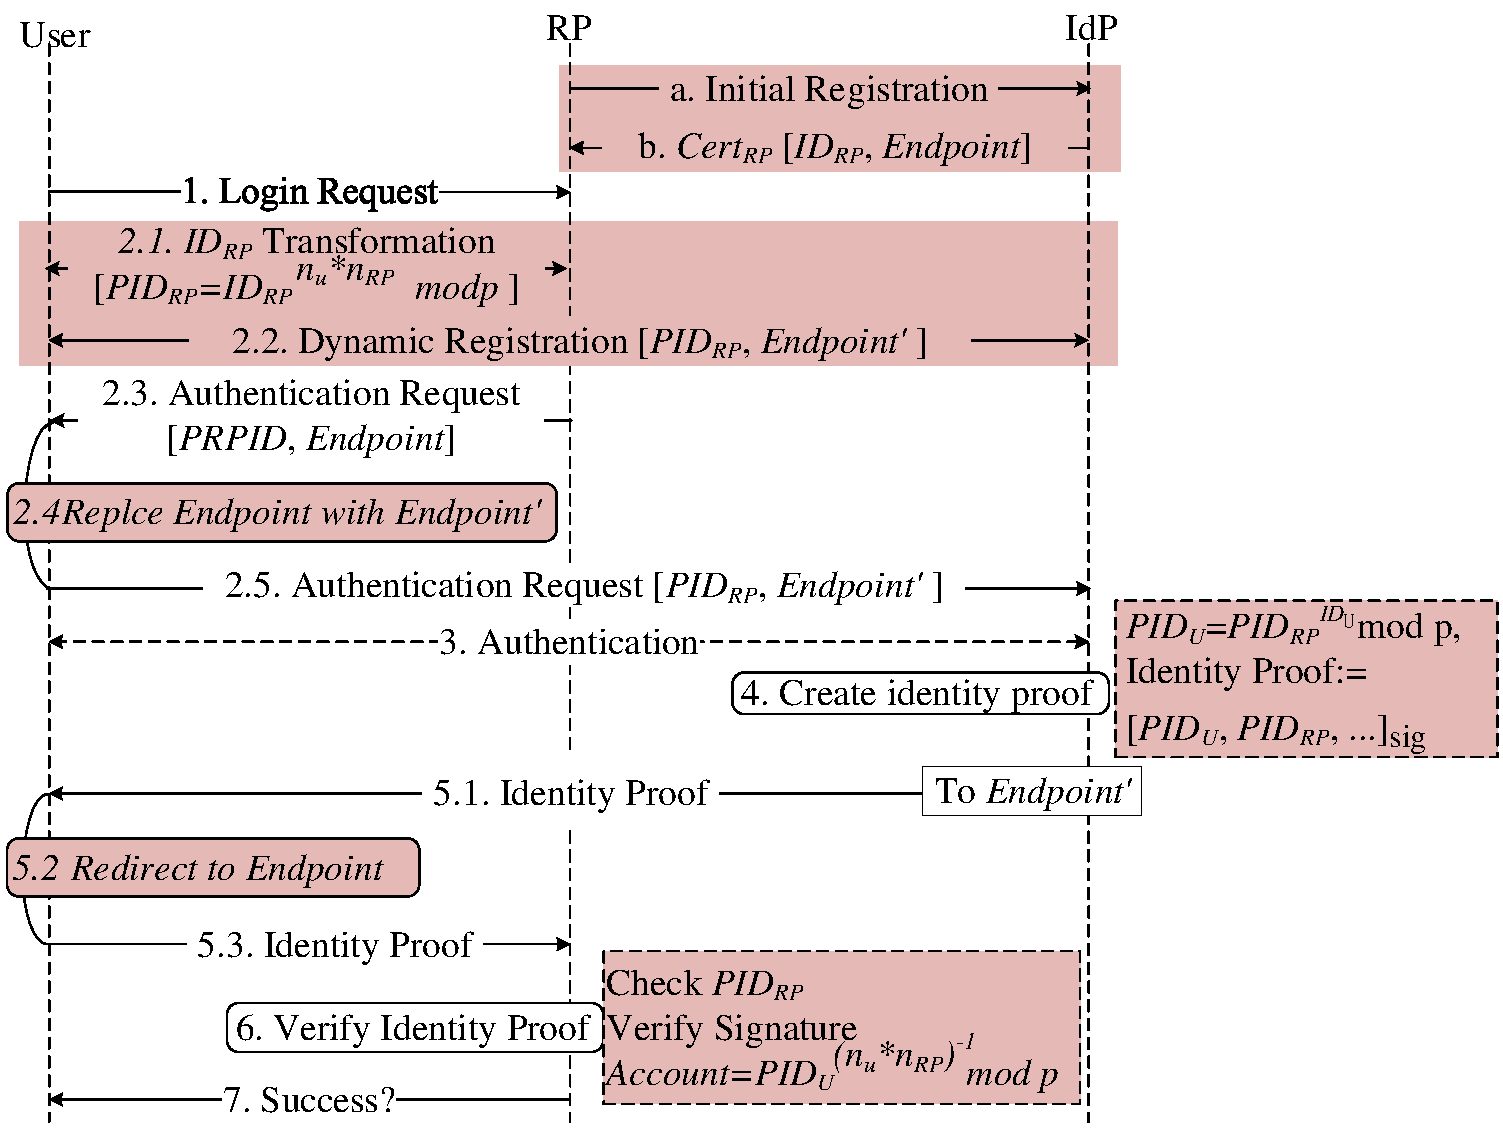
\includegraphics[width=\linewidth]{fig/overview1.pdf}
%  \caption{UPPRESSO compatibility with OIDC.}
%  \label{fig:UPPRESSO}
%\end{figure}
%

\end{comment}

\subsection{Compatibility with OIDC}
\label{subsec:compatible}
UPPRESSO does not introduce any new role nor change the security assumptions for each role. It follows a similar logic flow as OIDC in SSO login and only requires small modifications to perform identifier transformation.
%Here, we explain the modification in each of the five phases of its SSO login flow to show that UPPRESSO is compatible with OIDC, which indicates UPPRESSO can be easily integrated with other commonly used SSO systems.
Among the five phases, the {\em scripts downloading} and {\em RP identifier transformation} phases are newly introduced by UPPRESSO. The browser is required to download two scripts from the IdP and RP and most of the designed operations in these two phases are performed by the scripts in the browser. So, we require minimal modifications to the IdP and RP servers providing new network interfaces (i.e., the new URLs for downloading resources). The other three phases adopt a similar communication pattern as OIDC. In particular, the {\em $PID_{RP}$ registration} phase can be viewed as a variant of the RP dynamic registration flow of OIDC~\cite{DynamicRegistration}, which allows an entity to register its identity and endpoint at the IdP.
%Different from OIDC in which only RPs can call a dynamic registration, UPPRESSO allows any authenticated user to launch this process and register an RP identifier with the IdP.
%The {\em identity proof generation} and {\em $Account$ calculation} phases adopt the same steps and functions as the implicit protocol flow of OIDC, while using a few different parameters. First, in identity proof generation, $PID_U$ transformed from $ID_U$ is used to replace $ID_U$, which is directly supported by OIDC, similar as in the PPID approaches that also convert $ID_U$ into $PID_U$. The calculation of $Account$ from $PID_U$ 
%can be viewed as a customized step by the RP to derive its user account after the implicit protocol flow of OIDC ends.

%So,the identity proof generation and $Account$ calculation phases of UPPRESSO can be viewed as a particular but compatible implementation of the implicit protocol flow of OIDC. It is worth noting that the identity proof generation and $Account$ calculation phases of 
UPPRESSO can also support the authorization code flow of OIDC with small modifications (to be discussed in Section~\ref{sec:discussion}).

%As shown in Figure~\ref{fig:process}, in UPPRESSO, the SSO protocol for identity proof is the same as in OIDC; the formats of identity proof and corresponding request are the same as in OIDC; the correctness checks on the identity proof request at the IdP (i.e., consistency of RP' identifier and endpoint with the registered one) are the same as in OIDC; the correctness checks on the identity proof (i.e., consistency of RP' identifier with the one in the request, integrity, validity time, freshness, and etc.) at the RP are the same as in OIDC.
%The above modifications could be completed automatically for each login, without affecting other communication pattern.

%以下为描述Step 2.3到7的详细内容.
%That is, the RP construct a request for identity proof (Step 2.3); the user redirects this request to the IdP (Step 2.5); the IdP generates the identity proof (Step 4), and sends it to the user (Step 5.1) who redirects it to the RP (Step 5.3); and finally the RP verifies the identity proof (Step 6).

%However, UPPRESSO achieves privacy preservation by integrating  $\mathcal{F}_{ID_{U} \mapsto PID_{U}}$, $\mathcal{F}_{ID_{RP} \mapsto PID_{RP}}$ and $\mathcal{F}_{PID_{U} \mapsto Account}$, and  introduces the following modifications on OIDC.

%\begin{enumerate}
%  \item The identity proof is bound with $PID_{RP}$ instead of $ID_{RP}$, which introduces the RP identifier transforming (Steps 1.2-1.5)  and $PID_{RP}$ registration (Steps 2.1-2.4).
%  \item The identity proof is designated to one-time endpoint instead of RP's identifying endpoint, which requires the user to register the one-time endpoint in Step 2.1 and replace it with the original endpoint in Step 3.2.
%  \item IdP generates $PID_U$ based on ($PID_{RP}$, $ID_U$) instead of ($ID_{RP}$, $ID_U$).
%  \item The RP calculates $Account$ from the changing $PID_U$ instead of an unchanged one.
%\end{enumerate}

%上述modification如何实现的,简单描述
%to add: PID_{RP} transforming 和 RP identifer refreshing在user和RP的页面自己完成了。 都用现成的数据格式
%one-time endpoint 和endpoint
%The user automatically invokes the JavaScript functions to complete RP identifier transforming, one-time endpoint generating/replacing and $PID_{RP}$ registration for each login.
%While, the RP server and IdP server provide the corresponding web service to complete the processing automatically.

%The protocol of RP identifier transformation is based Diffie-Hellman key exchange~\cite{DiffieH76}, while $N_U$ is provided to RP for computing the trapdoor and $N_{RP}$ is provided to the user for verifying the correctness of $Y_{RP}$.

\begin{comment}
\vspace{1mm}\noindent \textbf{Consistency with OIDC.}
As shown in Figure~\ref{fig:UPPRESSO}, the architecture of UPPRESSO is the same as the one in OIDC. UPPRESSO does not introduce any new entity, but only integrates the three function $\mathcal{F}_{ID_{U} \mapsto PID_{U}}$, $\mathcal{F}_{ID_{RP} \mapsto PID_{RP}}$ and $\mathcal{F}_{PID_{U} \mapsto Account}$ into the processes at the IdP, RP, and user.

The formats of the  identity proof and corresponding request, and the verification of the identity proof,  are almost same in OIDC and UPPRESSO.
The only difference is that $ID_{RP}$ and endpoint are replaced with the privacy-preserving versions, i.e., $PID_{RP}$ and one-time endpoint, in UPPRESSO.
As $PID_{RP}$ is also unique and corresponds exactly to $ID_{RP}$, and one-time endpoint corresponds to the RP's endpoint correctly,
 the binding, integrity and confidentiality of identity proof will also be ensured in UPPRESSO, and there is no degradation on the security of OIDC.

\vspace{1mm}\noindent \textbf{Minimal modification to OIDC.}
UPPRESSO only requires small modification on OIDC to integrate $\mathcal{F}_{ID_{U} \mapsto PID_{U}}$, $\mathcal{F}_{ID_{RP} \mapsto PID_{RP}}$ and $\mathcal{F}_{PID_{U} \mapsto Account}$.
For $\mathcal{F}_{ID_{U} \mapsto PID_{U}}$ and $\mathcal{F}_{PID_{U} \mapsto Account}$, we directly use them to replace original functions for $PPID$ at the IdP and the $Account$ at the RP.
For $\mathcal{F}_{ID_{RP} \mapsto PID_{RP}}$, we inject a negotiation process and a dynamic registration for each SSO login,
 where the negotiation process between the user and RP generates a $PID_{RP}$,
  while the dynamic registration is used to check the uniqueness of $PID_{RP}$.
In UPPRESSO, the dynamic registration is slightly modified as follows: an RP identifer ($PID_{RP}$)  is added in the request, and a signature ($Sig_{Res}$)  is included in the response for its verification at the RP.
\end{comment}
